\documentclass[10 pt,usenames,dvipsnames, oneside]{article}
\usepackage{../../../modelo-ensino-medio}



\begin{document}

\begin{center}
  \begin{minipage}[l]{3cm}

\includegraphics[width=2cm]{logo}    
\end{minipage}\hfill
\begin{minipage}[r]{.8\textwidth}
 {\Large \scshape Atividade: 0,9999...}  
\end{minipage}
\end{center}
\vspace{.2cm}

\ifdefined\prof
%Habilidades da BNCC
\begin{objetivos}
\item \textbf{EM13MAT508} Identificar e associar progressões geométricas (PG) a funções exponenciais de domínios discretos, para análise de propriedades, dedução de algumas fórmulas e resolução de problemas.
\end{objetivos}

%Caixa do Para o Professor
\begin{goals}
%Objetivos específicos
\begin{enumerate}
\item Relacionar a soma da PG infinita com a representação decimal de um número real.
\end{enumerate}

\tcblower

%Orientações e sugestões
\begin{itemize}
\item O que é feito nessa atividade pode ser generalizado para a representação decimal de qualquer número real e o fato de podermos somar a PG infinita de razão $\frac 1{10}$ é o que garante que podemos escrever os famosos "três pontinhos" no final de cada número.
\end{itemize}
\end{goals}

\bigskip
\begin{center}
{\large \scshape Atividade}
\end{center}
\fi

O número $0,9999\ldots$ é uma dízima periódica, ou seja, é um número que apresenta um sequência infinita de algarismos decimais que se repetem. De um modo geral esses algarismos que se repetem - e que podem aparecer em grupos de um ou mais algarismos - ordenados sempre na mesma disposição é chamado de período da dízima. Uma outra notação muito utilizada consiste em pôr um traço sobre o período. Veja alguns exemplos:

\[
0{,}333333\ldots = 0,\overline{3} \,\ \,\ \,\   0{,}142857142857\ldots = 0{,}\overline{142857} \,\ \,\ \,\ 0{,}99999\ldots = 0{,}\overline{9}
\]

\begin{enumerate}

\item{}
Posicione o número $0,\overline{9}$ na reta real abaixo.

\begin{figure}[H]
\centering
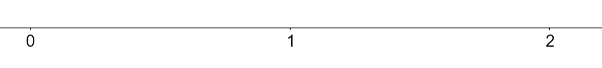
\includegraphics[width=400bp]{reta01.png}
\end{figure}

\item{}
Considere a progressão geométrica $(0{,}9; 0{,}09; 0{,}009; 0{,}0009; \ldots )$. Trata-se de uma sequência crescente ou decrescente? Qual a razão dessa PG?

\item{}
Que relação que a PG tem com o número $0,\overline{9}$?

\item{}
É possível calcular a soma de todos os infinitos termos dessa progressão? Caso positivo, calcule.

\item{}
Você mudaria a resposta que deu no item (a)?

\end{enumerate}

\ifdefined\prof
\clearpage
\begin{solucao}

\begin{enumerate}
\item {} Coincidindo com o número $1$.
	
\item{} Uma PG decrescente de razão $0{,}1$.
	
\item{} $0,\overline{9}=0{,}9+ 0{,}09+0{,}009+0{,}0009+\cdots$ é igual à soma infinita da PG.

\item{} 
%	PARA ESSE COMANDO CANCEL FUNCIONAR PRECISA DO PACOTE \usepackage{cancel}	
\begin{tabular}{ccccc}
\  & $S$ & = & $0{,}9+\cancel{0{,}09}+\cancel{0{,}009}+\cancel{0{,}0009}+\cdots$ & \ \\
$-($ & $0{,}1\cdot S$  & = & $\cancel{0{,}09}+\cancel{0{,}009}+\cancel{0{,}0009}+\cancel{0{,}00009}+\cdots$  & ) \\
\midrule
\  & $0{,}9\cdot S$ & = & $ 0{,}9 $ & \ \\
\end{tabular}

Portanto $S=1$

\item{} Resposta pessoal.		
\end{enumerate}

\end{solucao}
\fi

\end{document}